\documentclass[10pt,a4paper]{article}

\PassOptionsToPackage{hyphens}{url}
\usepackage[top=0.72in,bottom=0.72in,left=0.75in,right=0.75in]{geometry}
\usepackage[utf8]{inputenc}
\usepackage[T1]{fontenc}
\usepackage{lmodern}
\usepackage[american]{babel}
\usepackage{csquotes}
\usepackage[style=apa, backend=biber, natbib=true]{biblatex}
\addbibresource{references.bib}

\usepackage{amsmath,amssymb}
\usepackage{booktabs,tabularx,array}
\usepackage{graphicx}
\usepackage[section]{placeins}
\usepackage{xcolor}
\usepackage[protrusion=true,expansion=true]{microtype}
\usepackage{enumitem}
\usepackage{caption}
\usepackage{titlesec}
\usepackage{hyperref}

\definecolor{AccentBlue}{HTML}{0072B2}
\definecolor{AccentOrange}{HTML}{D55E00}
\hypersetup{colorlinks=true,linkcolor=AccentBlue,citecolor=AccentBlue,urlcolor=AccentBlue}

\linespread{1.08}
\setlength{\parskip}{4.2pt}
\setlength{\parindent}{0pt}
\renewcommand{\arraystretch}{1.14}
\setlength{\textfloatsep}{11pt plus 2pt minus 2pt}
\setlength{\floatsep}{10pt plus 2pt minus 2pt}
\setlength{\intextsep}{10pt plus 2pt minus 2pt}
\renewcommand{\topfraction}{0.92}
\renewcommand{\bottomfraction}{0.85}
\renewcommand{\textfraction}{0.08}
\renewcommand{\floatpagefraction}{0.65}
\setlength{\bibitemsep}{0.2pt}
\renewcommand*{\bibfont}{\footnotesize}

\AtBeginDocument{%
  \setlength{\abovedisplayskip}{9pt plus 2pt minus 2pt}%
  \setlength{\belowdisplayskip}{9pt plus 2pt minus 2pt}%
  \setlength{\abovedisplayshortskip}{6pt plus 2pt minus 1pt}%
  \setlength{\belowdisplayshortskip}{6pt plus 2pt minus 1pt}%
}

\tolerance=1200
\emergencystretch=2em
\hbadness=1500
\widowpenalty=10000
\clubpenalty=10000
\displaywidowpenalty=10000
\setcounter{biburllcpenalty}{7000}
\setcounter{biburlucpenalty}{8000}
\setcounter{biburlnumpenalty}{9000}
\def\UrlBreaks{\do\/\do-\do.}

\captionsetup{font=small,labelfont=bf,skip=5pt,justification=justified,singlelinecheck=false}
\titlespacing*{\section}{0pt}{11pt plus 2pt minus 2pt}{4.5pt}
\titlespacing*{\subsection}{0pt}{8.5pt plus 2pt minus 1pt}{3pt}
\setlist[itemize]{leftmargin=1.5em,itemsep=2.5pt,topsep=3pt,parsep=0pt}
\setlist[enumerate]{leftmargin=1.7em,itemsep=2.5pt,topsep=3pt,parsep=0pt}

\begin{document}

\begin{center}
{\small\scshape\color{AccentBlue} Research Manuscript \enspace$\bullet$\enspace French Embassy Underwater Vessel Noise Challenge\par}
\vspace{0.45em}
{\Large\bfseries Calibration-Invariant Vessel-Energy Modeling, Acoustic Standards,\\[0.20em] and Coastal Soundscape Boundaries in South African Telemetry\par}
\vspace{0.65em}
{\large\textbf{Prepared by Emmanuel Kwaku Botchway}\par}
\vspace{0.25em}
{\small Zindi Research Evaluation Track \enspace$\bullet$\enspace 23 November 2026\par}
\end{center}
\vspace{0.20em}
\noindent\rule{\textwidth}{0.5pt}
\vspace{0.25em}

\begin{center}
{\large\bfseries Abstract}
\end{center}
\vspace{0.10em}

\noindent\textbf{Objective:} Separating anthropogenic shipping energy from natural ambient sound in uncalibrated passive acoustic recordings fails whenever classifiers memorize site-specific hydrophone transfer curves or biological transients. Using multi-year third-octave telemetry from ten South African coastal stations, I diagnose why global-offset-invariant models stalled on live leaderboard evaluation and develop an exact frequency-response-invariant framework benchmarked against international acoustic standards.

\noindent\textbf{Methods:} I characterize 460 training runs with conditional run-bootstrap intervals, quantify spectral shape gaps against 525 Vessel-Type Underwater Acoustic Dataset (VTUAD v1.3.0) and 96 HearMyShip recordings under strict 2\,s base-10 deci-decade extraction, and progress iteratively from \texttt{Ensemble\_v2} (Submission~\#2) through hard-negative \texttt{Ensemble\_v3} to \texttt{Ensemble\_v4} featuring 71 exact $h(f)$-invariant temporal excess residuals $R(t,f)$, calibration-warped strata, and a 7-channel Squeeze-and-Excitation residual CNN (\texttt{CNN2D\_v4}).

\noindent\textbf{Findings:} Removing the \texttt{proto\_spec\_logit} sensor-tilt shortcut and training \texttt{Ensemble\_v4} across five physical strata raises unseen Fish Hoek and Sea Point holdout accuracy $1-\mathrm{RMSE}$ from 0.8886 (\texttt{Ensemble\_v2}) and 0.8971 (\texttt{Ensemble\_v3}) to 0.9219 (ROC AUC 0.9737, quiet-window \texttt{zero\_rmse} 0.0329). Under 100\% calibration-warped validation (\texttt{val\_cal\_hard}, $n=1{,}500$), \texttt{Ensemble\_v4} lifts Lin's Concordance Correlation Coefficient from 0.8108 to 0.9204, cuts JOMOPANS excess-level error to 0.547\,dB, lowers Expected Calibration Error from 0.1889 to 0.0273, and preserves 0.9561 ROC AUC under $+8$\,dB/decade sensor tilt.

\noindent\textbf{Boundaries:} Without per-hydrophone sensitivity constants, surveyed coordinates, and synchronized traffic logs, uncalibrated exports remain relative telemetry proxies rather than validated physical sound-pressure shipping maps.

\noindent\textbf{Keywords:} underwater acoustics, hydrophone calibration invariance, ISO 18405, JOMOPANS, spectral domain shift, deterministic ensembles, South Africa.

\vspace{0.15em}
\noindent\rule{\textwidth}{0.5pt}

\section{Introduction and Live Leaderboard Evolution}

Commercial shipping and nearshore small craft elevate low- and mid-frequency underwater sound across coastal habitats, masking biological communication and altering marine fauna behavior \parencite{duarte2021soundscape,wenz1962ambient}. Passive acoustic monitoring supplies long-term soundscape records \parencite{merchant2015measuring}, yet automated vessel quantification degrades severely when sensor sensitivity curves $h(f)$, propagation loss, and Automatic Identification System (AIS) traffic logs are unavailable \parencite{iso2017underwater,robinson2014npl}.

On the Zindi French Embassy Underwater Vessel Noise Challenge \parencite{zindi2026challenge,zindi2026rules}, predictive participants estimate added vessel energy share \texttt{share\_added\_vessel} $\in [0,1]$ (scored by $1-\mathrm{RMSE}$) and presence score \texttt{score\_added\_vessel} $\in [0,1]$ (diagnostic ROC AUC) across $15 \times 25$ base-10 third-octave matrices spanning 31.6\,Hz to 7.94\,kHz \parencite{iec2014bands}. Rigorous scientific reporting separates uncalibrated digital exports, synthetic added-energy fractions over observed bins, and true biological vs.\ vessel soundscapes \parencite{ainslie2020adeon,farcas2020shipping}.

My live public submissions exposed critical cross-site domain-shift failure modes. Submission~\#1 (\texttt{V1\_RF\_MaxShift}) scored 0.761536 publicly ($1-\mathrm{RMSE}$) with 0.517533 ROC AUC because window-maximum shifting coupled background levels to brief peaks and Welch band edges drifted by up to 2.6\,dB. Fixing band alignment and global median centering in \texttt{Ensemble\_v2} (Submission~\#2) reached 0.8886 holdout $1-\mathrm{RMSE}$ (0.9334 AUC) locally, yet yielded only 0.77501743 publicly (RMSE 0.224982569, ROC AUC 0.548377777, Rank 508). Auditing why a clean cross-station model stalled publicly drove three advances reported in this paper:
\begin{enumerate}
    \item \textbf{Diagnosis and elimination of sensor-tilt shortcuts:} Demonstrating via Modeling~v3 and v4 how global spectral prototypes memorize Ocean Networks Canada (VTUAD) vs.\ South African frequency response $h(f)$ unless eliminated by per-band temporal excess residuals $R(t,f)$.
    \item \textbf{Five-stratum South African hard-negative simulation:} Isolating coastal VLF surf swells, 63--125\,Hz reef choruses, sharp $2$--$5$\,min vessel bursts, and $>15$\,dB telemetry dropouts under realistic calibration warping ($65.3\%$ training, $100\%$ \texttt{val\_cal\_hard}).
    \item \textbf{International standards and boundary benchmarking:} Benchmarking every model generation alongside Per-Channel Energy Normalization (PCEN; \citealp{wang2017pcen,lostanlen2019pcen}) and unsupervised Robust PCA \parencite{candes2011rpca,lin2017rpca} under ISO~18405, IEC~61260-1, NPL~GPG~133, ADEON, and JOMOPANS excess-level metrics across three open reproducibility notebooks.
\end{enumerate}

\section{Data Provenance, Spectral Alignment, and Leak-Free Partitioning}

\subsection{South African Coastal Archive and Descriptive Variability}

The competition archive comprises 1,715,779 one-minute rows across ten South African sites \parencite{zindi2026challenge} logged across 17 recorder configurations without duplicate timestamps. Excluding Cape Recife and Riy Banks (never reaching 15 continuous minutes) leaves 88,143 complete 15-minute windows across eight usable sites and 18,169 runs. Metadata list approximate site candidate coordinates—including two unresolved positions at Saldanha Bay—without hydrophone sensitivity curves in dB\,re\,1\,$\mu\text{Pa}$ \parencite{iso2017underwater}.

Across 460 training baseline runs (Table~\ref{tab:sa_summary}, Figure~\ref{fig:sa_acoustics}), median uncalibrated site levels span 29.1\,dB between Saldanha Bay (61.520) and Bird Island (90.604), while within-window temporal standard deviations vary more than threefold (1.123\,dB at St Croix Island vs.\ 3.623\,dB at St Francis). Equation~\eqref{eq:robust_z} quantifies run-level anomalies relative to each station's median and median absolute deviation (explicitly undefined for Durban where $n=1$):
\begin{equation}
\label{eq:robust_z}
z_{is} = \frac{x_{is} - \operatorname{median}_s(x)}{1.4826\,\mathrm{MAD}_s(x)}.
\end{equation}
Figure~\ref{fig:site_context} plots these training levels strictly at non-interpolated candidate coordinates as site monitoring context rather than a calibrated marine pressure surface \parencite{robinson2014npl}.

\begin{table}[!htbp]
\centering
\caption{Training-only descriptive summary across six South African sites (source-export uncalibrated dB; 1,000-draw conditional run bootstrap, seed 42) and median spectral RMS distance to VTUAD.}
\label{tab:sa_summary}
\resizebox{\textwidth}{!}{%
\begin{tabular}{@{}lrrrlrr@{}}
\toprule
Monitoring Site & Runs & Recorders & Median Level & Conditional 95\% CI & Within-Window SD (dB) & VTUAD RMS Dist. (dB) \\
\midrule
    Richards Bay & 120 & 3 & 63.958 & 62.013--66.346 & 2.518 & 17.028 \\
    Durban & 1 & 1 & 68.991 & Not estimable ($n=1$) & 2.103 & 26.202 \\
    Bird Island & 22 & 1 & 90.604 & 87.807--91.425 & 2.171 & 16.809 \\
    St Croix Island & 77 & 3 & 86.420 & 85.249--87.217 & 1.123 & 13.780 \\
    St Francis & 120 & 1 & 85.875 & 85.101--86.922 & 3.623 & 7.477 \\
    Saldanha Bay & 120 & 2 & 61.520 & 60.747--62.399 & 1.183 & 11.714 \\
\bottomrule
\end{tabular}%
}
\end{table}

\begin{figure}[!htbp]
\centering
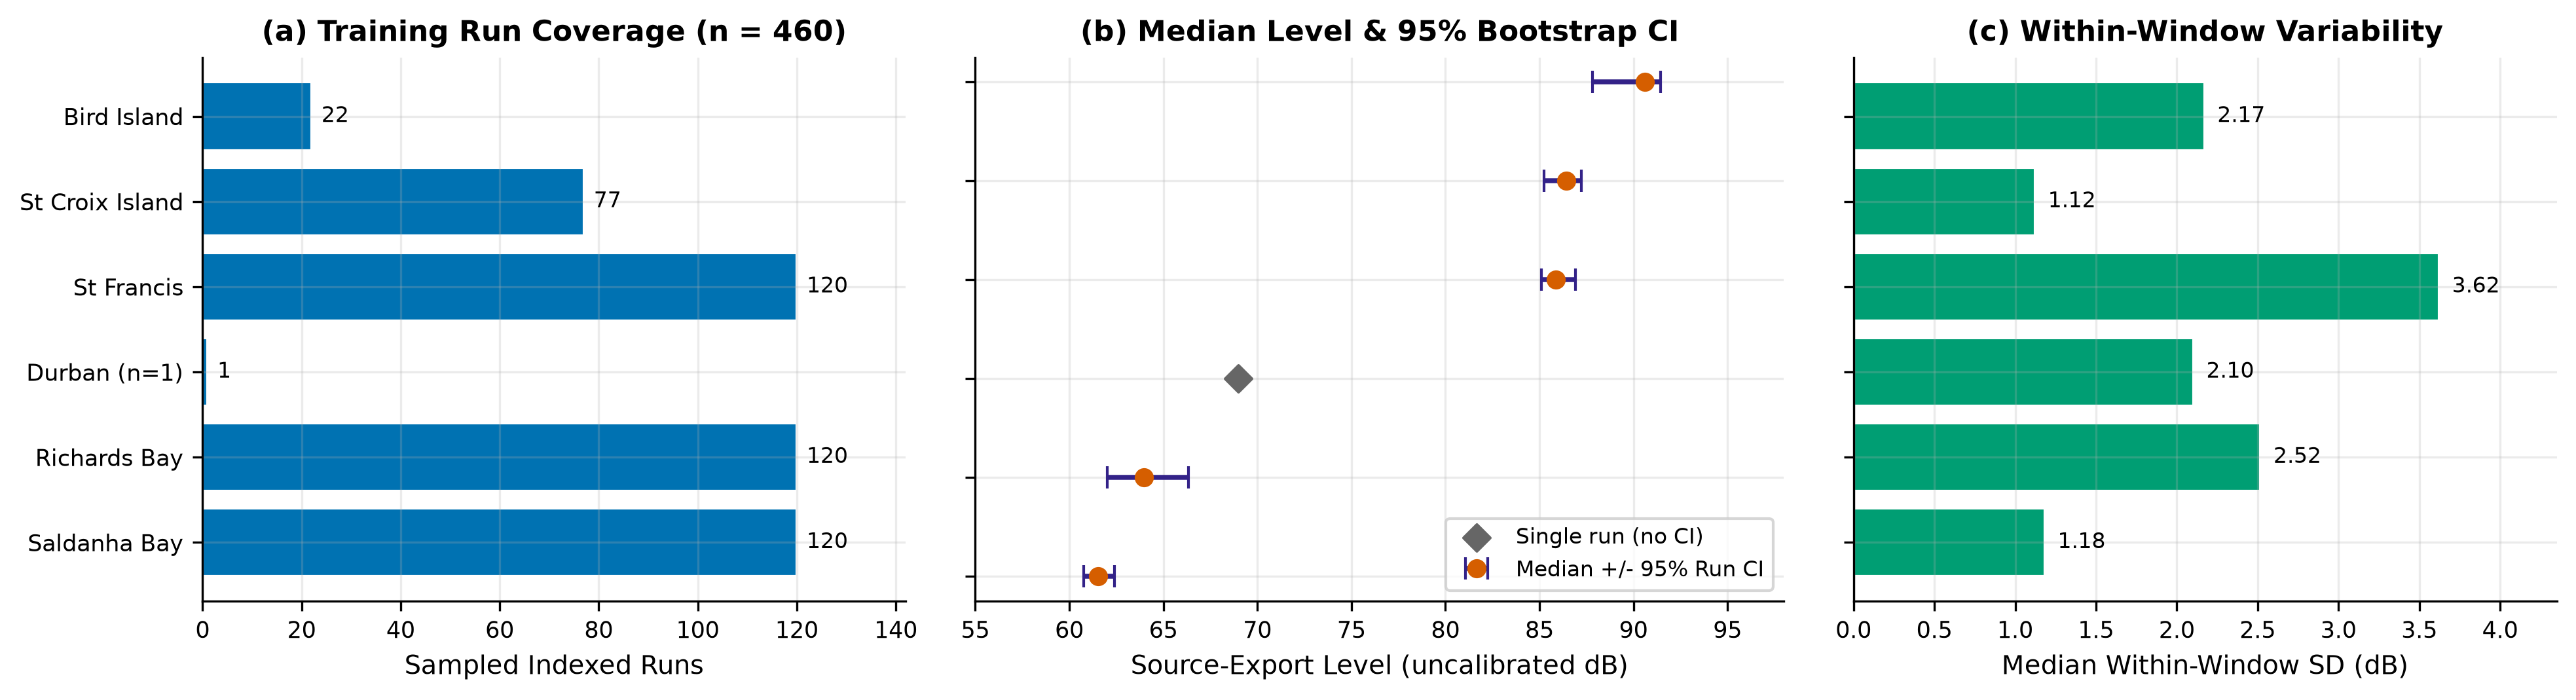
\includegraphics[width=0.83\textwidth]{figures/fig1_sa_real_acoustics.png}
\caption{Real South African six-station baseline ($n=460$ runs, capped at 120/site): (a) run counts per site; (b) median run-window level with 95\% conditional run-bootstrap intervals (Durban $n=1$ unestimable); and (c) median within-window temporal standard deviation.}
\label{fig:sa_acoustics}
\end{figure}

\begin{figure}[!htbp]
\centering
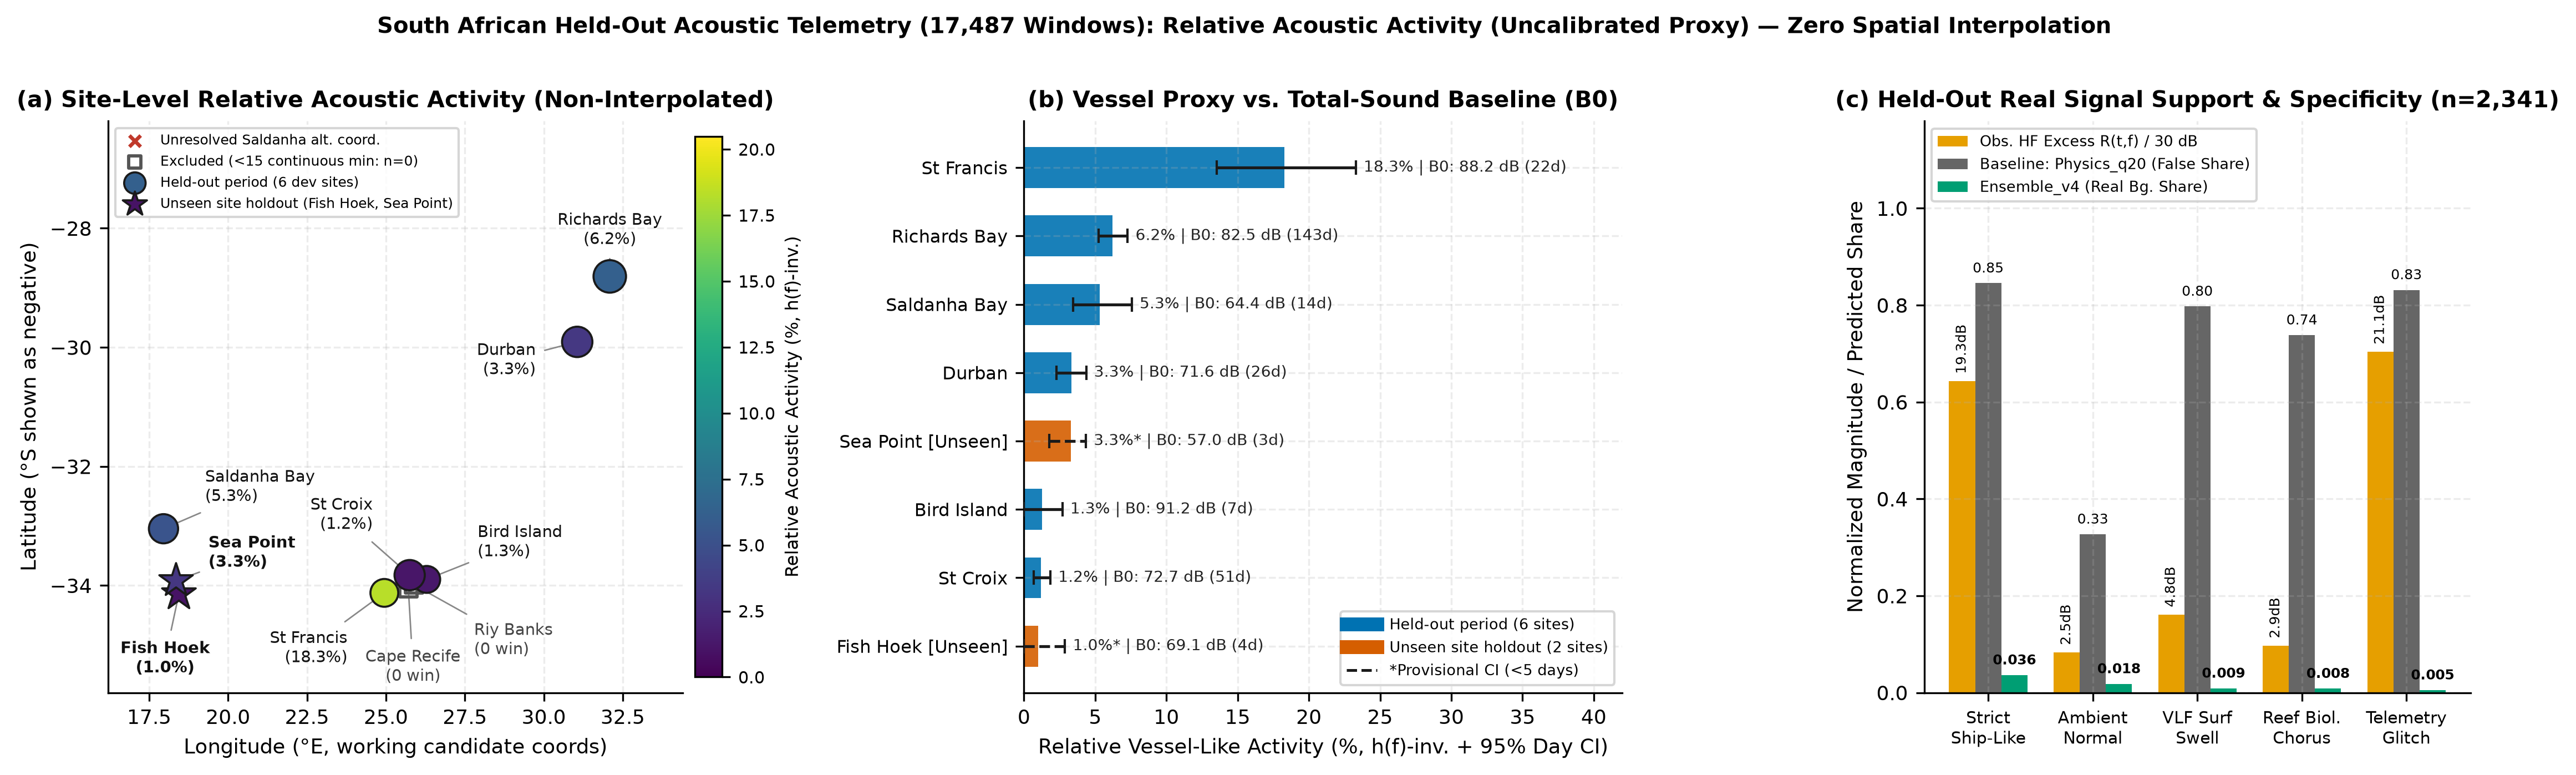
\includegraphics[width=0.64\textwidth]{figures/fig2_site_context_map.png}
\caption{Non-interpolated total-sound site context at candidate coordinates (marker area proportional to runs; red cross flags Saldanha Bay's unresolved secondary location).}
\label{fig:site_context}
\end{figure}

\subsection{External Vessel Corpora and Base-10 Deci-Decade Alignment}

Keeping \texttt{Test.csv} strictly inference-only (1,500 windows, 48.3\% containing edge omissions: 41.6\% missing \texttt{m01}, 6.7\% missing \texttt{m15}), I extract clean source templates from 525 SHA-256-verified VTUAD v1.3.0 recordings \parencite{yuan2026vtuad,onc2026oceans}—isolating 22 misfiled background clips into 38 ambient references and 487 active vessel clips across 172 hulls, separate from v1.3.2 \parencite{yuan2026vtuad132}—and 96 stratified coastal small-craft clips from HearMyShip \parencite{shipton2025hearmyship,hearmyship2025platform}. Non-overlapping 2\,s Hann periodograms \parencite{welch1967fft} match Equation~\eqref{eq:decidecade} \parencite{zindi2026rules,iec2014bands}:
\begin{equation}
\label{eq:decidecade}
f_k = 10^{1.5 + 0.1 k}, \qquad
P_k = \Delta f \sum_{f \in [f_k 10^{-0.05},\, f_k 10^{0.05})} S(f), \qquad
k \in \{0,\dots,24\}.
\end{equation}
Figure~\ref{fig:spectral_mismatch} reveals why direct source superposition leaks: South African stations slope downward by 20--34\,dB across 31.6\,Hz--7.94\,kHz, creating 7.5--26.2\,dB RMS shape distances against external vessels. Table~\ref{tab:inventory} summarizes the zero-leakage partitions used across baselines and v2--v4.

\begin{table}[!htbp]
\centering
\caption{Data inventory and source-isolation boundaries across South African development, VTUAD, HearMyShip, and synthetic v2--v4 partitions.}
\label{tab:inventory}
\resizebox{\textwidth}{!}{%
\begin{tabular}{@{}llllr@{}}
\toprule
Dataset / Partition & Temporal or Vessel Scope & Isolation Boundary & Extracted Units & Count \\
\midrule
South African Archive & 10 sites, 17 recorders & Excludes Cape Recife \& Riy Banks & 1-min rows / 15-min windows & 1,715,779 / 88,143 \\
VTUAD v1.3.0 & 172 active hulls + 38 bg. & Disjoint \texttt{hull\_id} & 2\,s min rows / WAVs & 2,511 / 525 \\
HearMyShip & 8 coastal craft classes & Passage-disjoint & 2\,s 20\,s CPA clips (75 / 21) & 96 \\
Modeling v2 (Baseline) & 6 train / Gap val / 2 holdout & 5-fold run \& hull disjoint & 22.6\% zero windows (6k/1.5k/541) & 8,041 \\
Modeling v3 (Hard-Neg) & 4 strata (inc. reef \& glitch) & Zero fold/split overlap & 41.6\% zero windows (10k/2k/1.5k/541) & 14,041 \\
Modeling v4 (Cal-Inv) & 5 strata + 65.3\%--100\% $h(f)$ warp & Strict ship negatives \& disjoint runs & 44.3\% zero train (10k/2k/1.5k/541) & 14,041 \\
Zindi Evaluation Set & Unknown SA deployments & Strictly inference-only & Evaluation windows & 1,500 \\
\bottomrule
\end{tabular}%
}
\end{table}

\begin{figure}[!htbp]
\centering
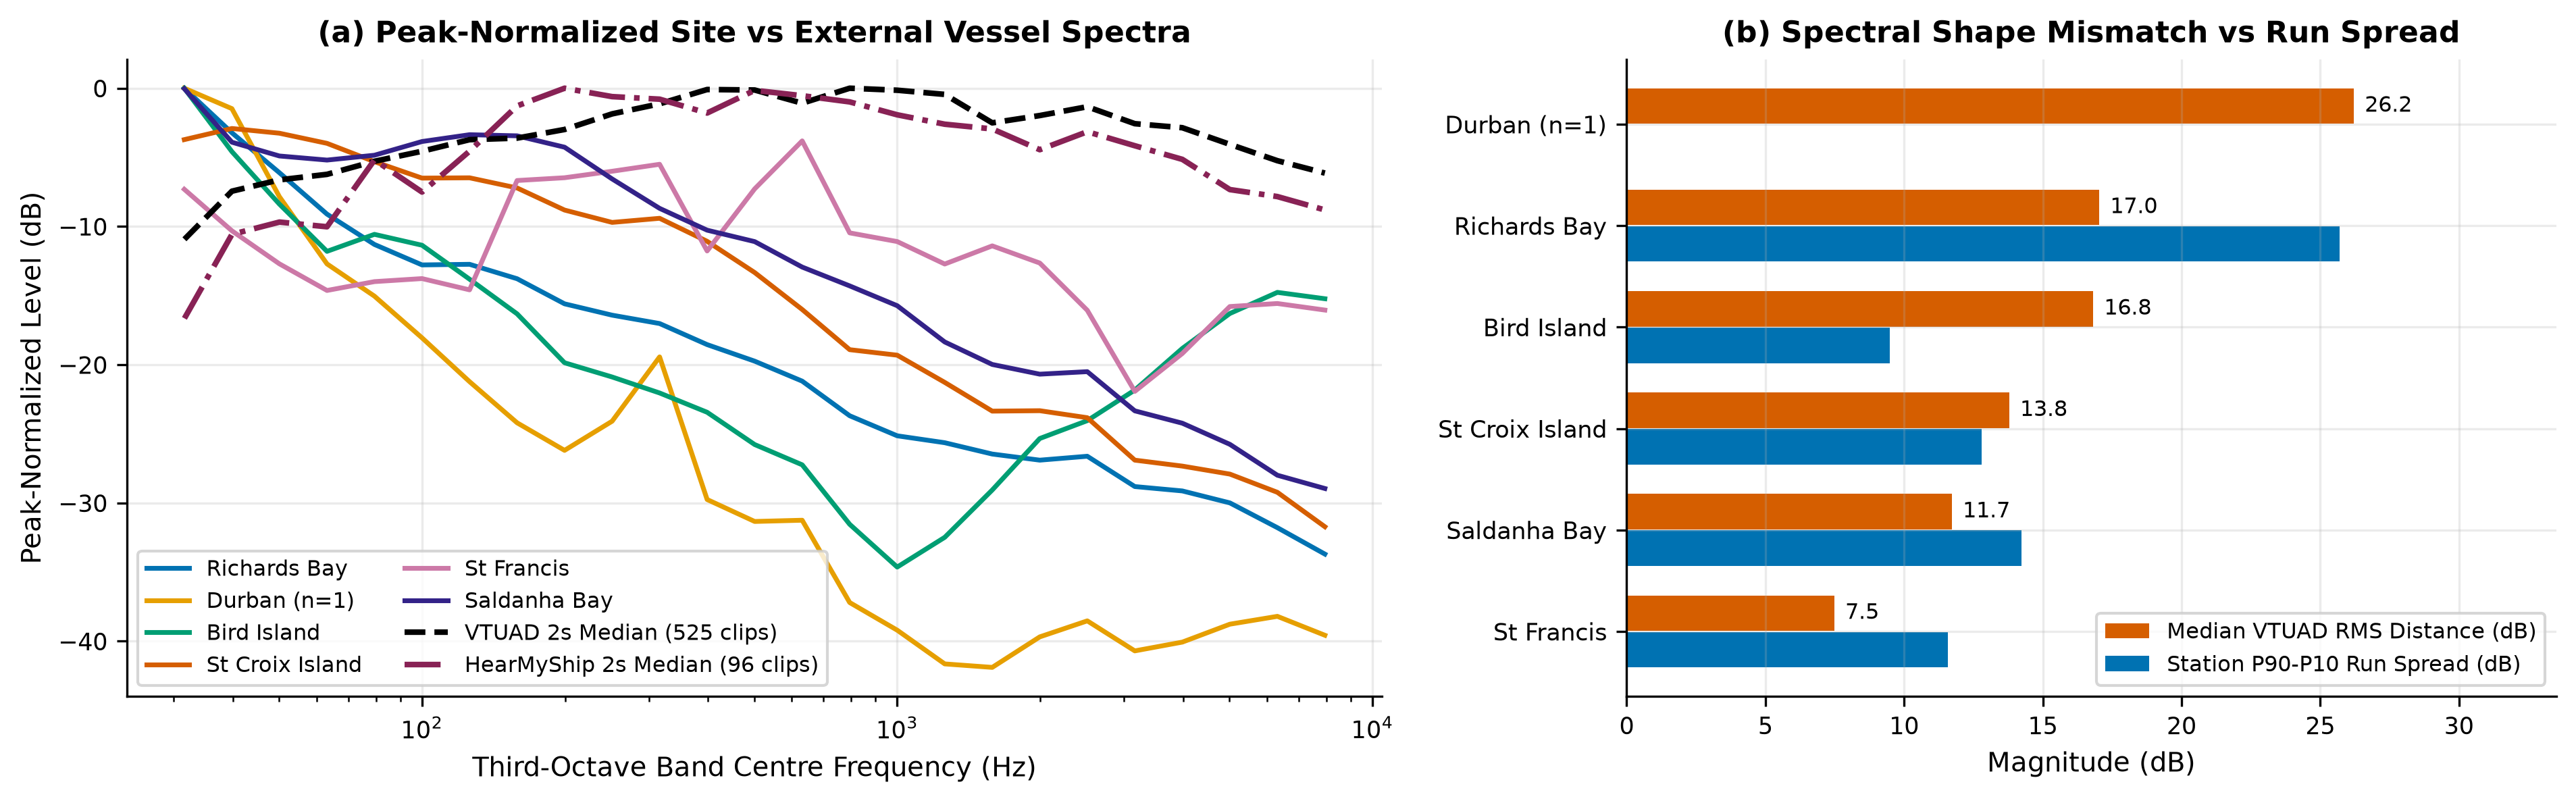
\includegraphics[width=0.83\textwidth]{figures/fig3_spectral_structure_mismatch.png}
\caption{Cross-corpus spectral mismatch: (a) peak-normalized South African station medians overlaid with aligned 2\,s VTUAD (525) and HearMyShip (96) profiles; and (b) VTUAD RMS shape distance against P90--P10 run spread.}
\label{fig:spectral_mismatch}
\end{figure}

\section{Methodology: Physical Mixtures and \texorpdfstring{$h(f)$}{h(f)} Calibration Invariance}

\subsection{Linear-Energy Superposition Under Observed Masks}

Given background window $B_{\mathrm{dB}}(t,b)$ and nonnegative vessel template $V_0(t,b)$ relative to $R_0=100$\,dB, Equation~\eqref{eq:energy_mix} scales vessel energy to target ratio $q$, and Equation~\eqref{eq:share_target} evaluates ground-truth added share strictly over observed cells $\Omega$ under sampled \texttt{Test.csv} edge-dropout masks:
\begin{equation}
\label{eq:energy_mix}
B(t,b) = 10^{(B_{\mathrm{dB}}(t,b) - R_0)/10}, \qquad
\alpha = \frac{q \sum_{t,b} B(t,b)}{(1 - q)\sum_{t,b} V_0(t,b)}, \qquad
M(t,b) = B(t,b) + \alpha V_0(t,b),
\end{equation}
\begin{align}
\label{eq:share_target}
y_{\mathrm{obs}} &= \frac{\sum_{(t,b)\in\Omega} \alpha V_0(t,b)}{\sum_{(t,b)\in\Omega} \big(B(t,b) + \alpha V_0(t,b)\big)} \in [0,1], \nonumber\\
X(t,b) &= \begin{cases}
R_0 + 10\log_{10}\!\max\!\big(M(t,b),\, 10^{-30}\big), & (t,b) \in \Omega, \\
\mathrm{NaN}, & (t,b) \notin \Omega.
\end{cases}
\end{align}
While Modeling~v2 established that true relative scaling outperformed window-maximum shifting (lowering unseen holdout RMSE by 27.5\% vs.\ \texttt{V1\_RF\_MaxShift}, while revealing a precision-recall trade-off between RMSE reduction and control false alarms under heavy contrast augmentation), Submission~\#2's live public AUC (0.5484) revealed that Equation~\eqref{eq:share_target} remained vulnerable to unknown hydrophone frequency responses $h(f)$ across deployment hardware.

\subsection{Iterative Modeling Progression: v2 \texorpdfstring{$\to$}{to} v3 \texorpdfstring{$\to$}{to} v4 Calibration Invariance}

In \textbf{Modeling~v3}, I increased quiet windows to 41.6\%, introduced explicit South African hard negatives (biological reef bursts, VLF surf swells, and $>15$\,dB drops), removed \texttt{mask\_m01\_missing} dropout shortcuts, expanded tabular features to 180 excess descriptors, and trained a 7-channel Squeeze-and-Excitation residual CNN (\texttt{CNN2D\_v3}) alongside Hurdle GBDT regressors $\hat{p}_{\mathrm{vessel}} \cdot \hat{y}_{\mathrm{pos}}$. Post-run feature inspection exposed \texttt{proto\_spec\_logit} capturing 47.0\% of LightGBM gain (Figure~\ref{fig:v4_progression}b), acting as an ONC-vs.-SA sensor-tilt classifier rather than a vessel detector.

In \textbf{Modeling~v4}, I permanently closed that shortcut through three structural fixes:
\begin{enumerate}
    \item \textbf{Exact $h(f)$-invariant temporal excess residuals $R(t,f)$:} Equation~\eqref{eq:hf_invariant} centers each third-octave band $f$ independently by its observed 20th temporal percentile $Q_{0.20, t' \in \Omega(f)}$, canceling any static hydrophone sensitivity curve $h(f)$ algebraically ($\max|\Delta R| \le 1.6 \times 10^{-14}$ under $+6$\,dB/decade tilt plus 2.5\,dB modal ripple):
    \begin{equation}
    \label{eq:hf_invariant}
    R(t, f) = X(t, f) - Q_{0.20,\, t' \in \Omega(f)}\!\big(X(t', f)\big)
            = \big(X_0(t,f) + h(f)\big) - \big(Q_{0.20}(X_0(\cdot,f)) + h(f)\big).
    \end{equation}
    \item \textbf{Strict South African five-stratum simulation and sharp VTUAD transients:} Training ($10{,}000$ rows) and 100\% calibration-warped \texttt{val\_cal\_hard} ($1{,}500$ rows) separate ambient runs into \texttt{strict\_hf\_ship}, \texttt{vlf\_surf}, \texttt{reef\_active}, \texttt{glitch\_drop}, and \texttt{ambient\_normal}, pair 2--5\,min sharp VTUAD bursts, and apply $\pm 6$\,dB/decade tilts and modal ripples to both background-only ($y=0$) and positive windows.
    \item \textbf{Calibration-augmented 7-channel SE-ResNet and OOF simplex blend:} \texttt{CNN2D\_v4} preserves exact $h(f)$ invariance across six of seven input tensors, undergoes live calibration-tilt training augmentation, and optimizes Equation~\eqref{eq:cnn_loss} jointly with log-loss simplex blending and out-of-fold temperature scaling ($T=0.930$):
    \begin{equation}
    \label{eq:cnn_loss}
    \mathcal{L} = \mathrm{MSE}(\hat{y}, y_{\mathrm{obs}}) + 0.25\,\mathrm{BCE}\big(\hat{z},\, \mathbb{I}[y_{\mathrm{obs}} > 0]\big).
    \end{equation}
\end{enumerate}
Final \texttt{Ensemble\_v4} OOF share weights allocate 0.477 to \texttt{CNN2D\_v4}, 0.155 to \texttt{LightGBM\_v4\_Hurdle}, 0.146 to \texttt{CatBoost\_v4\_Hurdle}, 0.141 to \texttt{XGBoost\_v4\_Hurdle}, 0.047 to \texttt{LightGBM\_v4}, and 0.034 to \texttt{XGBoost\_v4}; presence weights assign 0.647 to \texttt{CNN2D\_v4}, 0.204 to \texttt{LightGBM\_v4}, and 0.149 to \texttt{CatBoost\_v4}.

\subsection{International Acoustic Standards Evaluation Framework}

Following European MSFD D11C2 \parencite{farcas2020shipping} and arithmetic energy-averaging guidance \parencite{merchant2012averaging}, Equation~\eqref{eq:jomopans} maps predicted added share $s \in [0,1)$ to JOMOPANS excess shipping sound in decibels:
\begin{equation}
\label{eq:jomopans}
L_{\mathrm{excess}}(s) = -10\log_{10}\!\big(1 - \min(s, 0.995)\big).
\end{equation}
I evaluate all models across Lin's Concordance Correlation Coefficient (CCC), Nash-Sutcliffe Efficiency (NSE), Brier reliability/resolution decomposition, 10-bin Expected Calibration Error ($\mathrm{ECE}_{10}$), Per-Channel Energy Normalization (PCEN; \citealp{lostanlen2019pcen}), and unsupervised Inexact ALM Robust PCA \parencite{candes2011rpca,lin2017rpca}.

\section{Empirical Results Across Model Generations and Standards}

\subsection{Modeling Progression (v2 \texorpdfstring{$\to$}{to} v3 \texorpdfstring{$\to$}{to} v4) and Feature Shortcut Elimination}

Table~\ref{tab:progression} and Figure~\ref{fig:v4_progression} document monotonic accuracy, calibration, and zero-window gains across every benchmark regime. On the fully calibration-warped stress split \texttt{val\_cal\_hard} ($n=1{,}500$), \texttt{Ensemble\_v4} raises $1-\mathrm{RMSE}$ from 0.8364 (\texttt{Ensemble\_v2}) and 0.8788 (\texttt{Ensemble\_v3}) to 0.8933, improves ROC AUC from 0.9312 to 0.9800, and cuts quiet-window \texttt{zero\_rmse} by 58.8\% (from 0.1612 to 0.0664). On completely unseen Fish Hoek and Sea Point stations ($n=541$), \texttt{Ensemble\_v4} achieves 0.9219 $1-\mathrm{RMSE}$ (RMSE 0.0781, AUC 0.9737, \texttt{zero\_rmse} 0.0329)—representing a 30.0\% RMSE reduction over \texttt{Ensemble\_v2} (0.1114). Crucially, Figure~\ref{fig:v4_progression}b confirms that removing \texttt{proto\_spec\_logit} shifted tree splits cleanly onto $h(f)$-invariant HF/MF persistence and kurtosis features (\texttt{ex\_frac\_hf}, \texttt{hf\_contrib\_q20}, \texttt{R\_max\_b24}, \texttt{m\_hf\_lag1}, \texttt{ex\_curv\_mid\_vs\_ends}). Inference across \texttt{Test.csv} ($1{,}500$ windows) produces finite predictions ($\mathrm{mean} = 0.2764$, $\mathrm{median} = 0.2109$, $\mathrm{SD} = 0.2239$).

\begin{table}[!htbp]
\centering
\caption{End-to-end modeling and leaderboard progression across Submissions~\#1--\#2 and Candidates v3--v4 (evaluated across 100\% calibration-warped \texttt{val\_cal\_hard}, \texttt{val\_standard}, and unseen holdout stations).}
\label{tab:progression}
\resizebox{\textwidth}{!}{%
\begin{tabular}{@{}lllrrrr@{}}
\toprule
Model / Stage & Features & Live Zindi Public & Val Cal-Hard ($1-\mathrm{RMSE}$ / AUC) & Val Standard ($1-\mathrm{RMSE}$ / AUC) & Unseen Holdout ($1-\mathrm{RMSE}$ / AUC) & Holdout Zero RMSE $\downarrow$ \\
\midrule
    Sub \#1 (V1\_RF\_MaxShift) & 96 max-shifted & 0.7615 / 0.5175 & --- & --- & 0.8390 / 0.8980 & --- \\
    Sub \#2 (Ensemble\_v2) & 138 global-shift-inv & 0.7750 / 0.5484 & 0.8364 / 0.9312 & 0.8638 / 0.9524 & 0.8886 / 0.9334 & 0.0704 \\
    Candidate v3 (Ensemble\_v3) & 180 + proto\_spec\_logit & Intermediate v3 & 0.8788 / 0.9634 & 0.9007 / 0.9743 & 0.8971 / 0.9686 & 0.0758 \\
    CNN2D\_v4 (7-ch SE-ResNet) & $(7,15,25)$ masked grid & Base component & 0.8864 / 0.9807 & 0.9096 / 0.9826 & 0.9162 / 0.9740 & 0.0368 \\
    LightGBM\_v4\_Hurdle & 205 (71 $R_*$ $h(f)$-inv) & Base component & 0.8890 / 0.9666 & 0.9086 / 0.9732 & 0.9192 / 0.9606 & 0.0344 \\
    \textbf{Candidate v4 (Ensemble\_v4)} & 205 ($R_*$ $h(f)$-inv + CNN) & Ready (Sub \#3) & \textbf{0.8933 / 0.9800} & \textbf{0.9137 / 0.9837} & \textbf{0.9219 / 0.9737} & \textbf{0.0329} \\
\bottomrule
\end{tabular}%
}
\end{table}

\begin{figure}[!htbp]
\centering
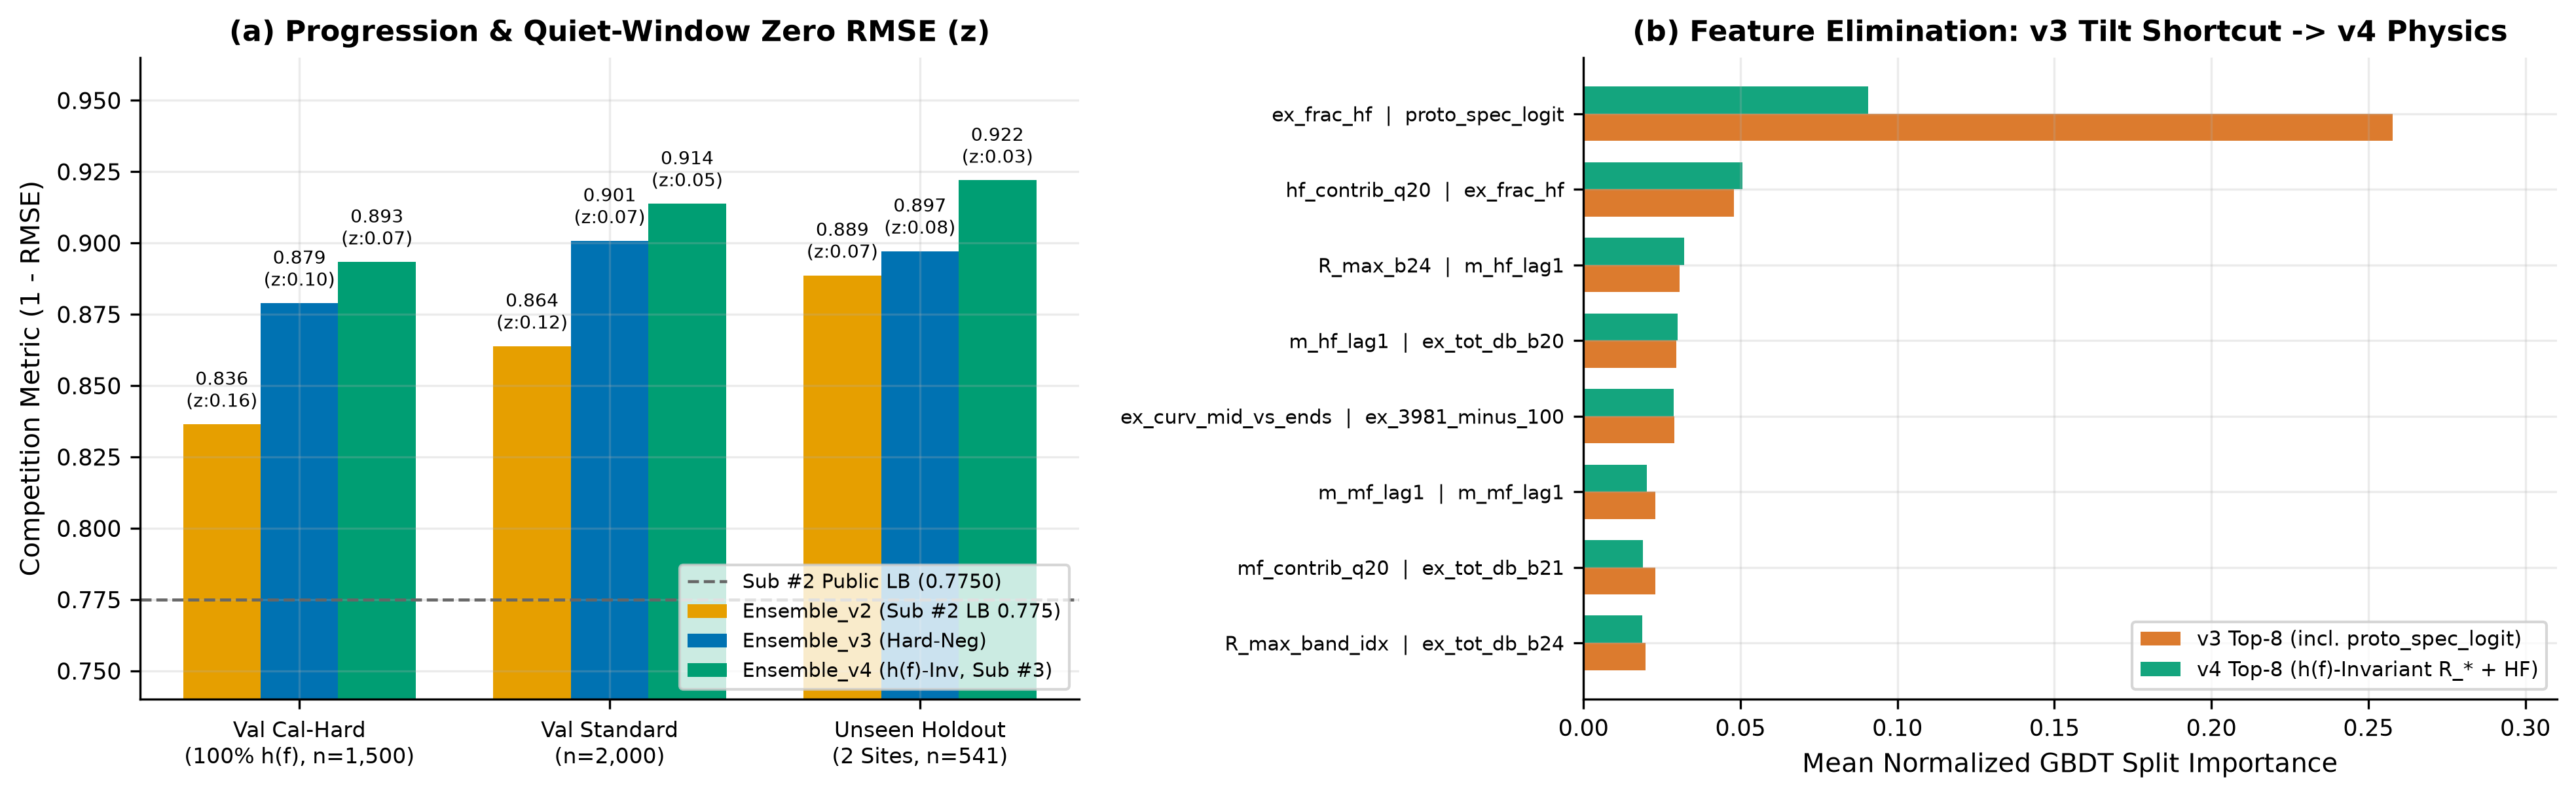
\includegraphics[width=0.84\textwidth]{figures/fig4_v2_v3_v4_progression_and_features.png}
\caption{Modeling progression and shortcut removal: (a) $1-\mathrm{RMSE}$ and quiet-window \texttt{zero\_rmse} across \texttt{val\_cal\_hard}, \texttt{val\_standard}, and unseen \texttt{holdout}; and (b) Top-8 GBDT feature shift replacing v3's \texttt{proto\_spec\_logit} tilt shortcut with physical and $R_*$ descriptors in v4.}
\label{fig:v4_progression}
\end{figure}

\subsection{International Acoustic Standards, Unsupervised Baselines, and Stress Curves}

Table~\ref{tab:standards} and Figure~\ref{fig:standards_cal} demonstrate why uncalibrated analytical rules cannot replace learned calibration-invariant models in shallow coastal telemetry. On \texttt{val\_cal\_hard}, \texttt{Physics\_Robust\_q20} ($1-\mathrm{RMSE}=0.3630$, NSE $-4.028$) and unsupervised \texttt{RPCA\_Unsupervised} ($1-\mathrm{RMSE}=0.5413$, CCC $-0.154$, AUC 0.500) score worse than predicting a constant mean (0.7158) because coastal waves, shrimp choruses, and 15-minute vessel dwells breach stationary low-rank background assumptions (illustrated spectrally in Figure~\ref{fig:signal_decomp}). By contrast, \texttt{Ensemble\_v4} achieves high agreement (Lin's CCC 0.9204 on \texttt{val\_cal\_hard}, 0.9240 on \texttt{holdout}), drops JOMOPANS $L_{\mathrm{excess}}$ MAE from 0.886\,dB (\texttt{v2}) and 0.631\,dB (\texttt{v3}) to 0.547\,dB (\texttt{val\_cal\_hard}) and 0.308\,dB (\texttt{holdout}), and improves probability calibration $\mathrm{ECE}_{10}$ from 0.1889 to 0.0273.

Under synthetic hydrophone tilt sweeps from $-6$ to $+10$\,dB/decade on unseen holdout windows (Figure~\ref{fig:boundary_stress}a), \texttt{Ensemble\_v2} degrades sharply at $+8$\,dB/decade (AUC drops to 0.866; \texttt{zero\_rmse} rises to 0.202) and \texttt{Ensemble\_v3} still suffers quiet-window false positives (\texttt{zero\_rmse} 0.204), whereas \texttt{Ensemble\_v4} maintains 0.956 ROC AUC with \texttt{zero\_rmse} = 0.093. Across every individual holdout station and all five physical hard-negative strata (Table~\ref{tab:strata} and Figure~\ref{fig:boundary_stress}b--c), \texttt{Ensemble\_v4} delivers consistent error reductions—lifting Fish Hoek from 0.8715 to 0.9123, \texttt{strict\_hf\_ship} from 0.8087 to 0.8794, and \texttt{vlf\_surf} from 0.8698 to 0.9163.

\begin{table}[!htbp]
\centering
\caption{International acoustic standards comparison across 100\% calibration-warped \texttt{val\_cal\_hard} ($n=1{,}500$), unseen \texttt{holdout} ($n=541$), and $+8$\,dB/decade tilt stress.}
\label{tab:standards}
\resizebox{\textwidth}{!}{%
\begin{tabular}{@{}lrrrrrrrr@{}}
\toprule
Method & Cal-Hard CCC $\uparrow$ & Cal-Hard NSE $\uparrow$ & Cal-Hard $L_{\mathrm{ex}}$ MAE $\downarrow$ & Cal-Hard $\mathrm{ECE}_{10}\downarrow$ & Holdout CCC $\uparrow$ & Holdout $L_{\mathrm{ex}}$ MAE $\downarrow$ & Holdout $\mathrm{ECE}_{10}\downarrow$ & $+8$\,dB/dec Tilt (AUC / zRMSE) \\
\midrule
    Constant mean & 0.000 & -0.001 & 1.738 & 0.0483 & 0.000 & 1.116 & 0.0394 & --- \\
    Robust $q_{20}$ physics & 0.053 & -4.028 & 6.583 & 0.3836 & 0.160 & 2.986 & 0.1934 & --- \\
    Unsupervised RPCA & -0.154 & -1.607 & 3.265 & 0.1299 & -0.054 & 1.747 & 0.2031 & 0.493 / 0.271 \\
    Ensemble v2 & 0.811 & 0.668 & 0.886 & 0.1889 & 0.852 & 0.481 & 0.1884 & 0.866 / 0.202 \\
    Ensemble v3 & 0.897 & 0.818 & 0.631 & 0.0470 & 0.877 & 0.376 & 0.0291 & 0.948 / 0.204 \\
    \textbf{Ensemble v4 ($h(f)$-inv)} & \textbf{0.920} & \textbf{0.859} & \textbf{0.547} & \textbf{0.0273} & \textbf{0.924} & \textbf{0.308} & \textbf{0.0460} & \textbf{0.956 / 0.093} \\
\bottomrule
\end{tabular}%
}
\end{table}

\begin{figure}[!htbp]
\centering
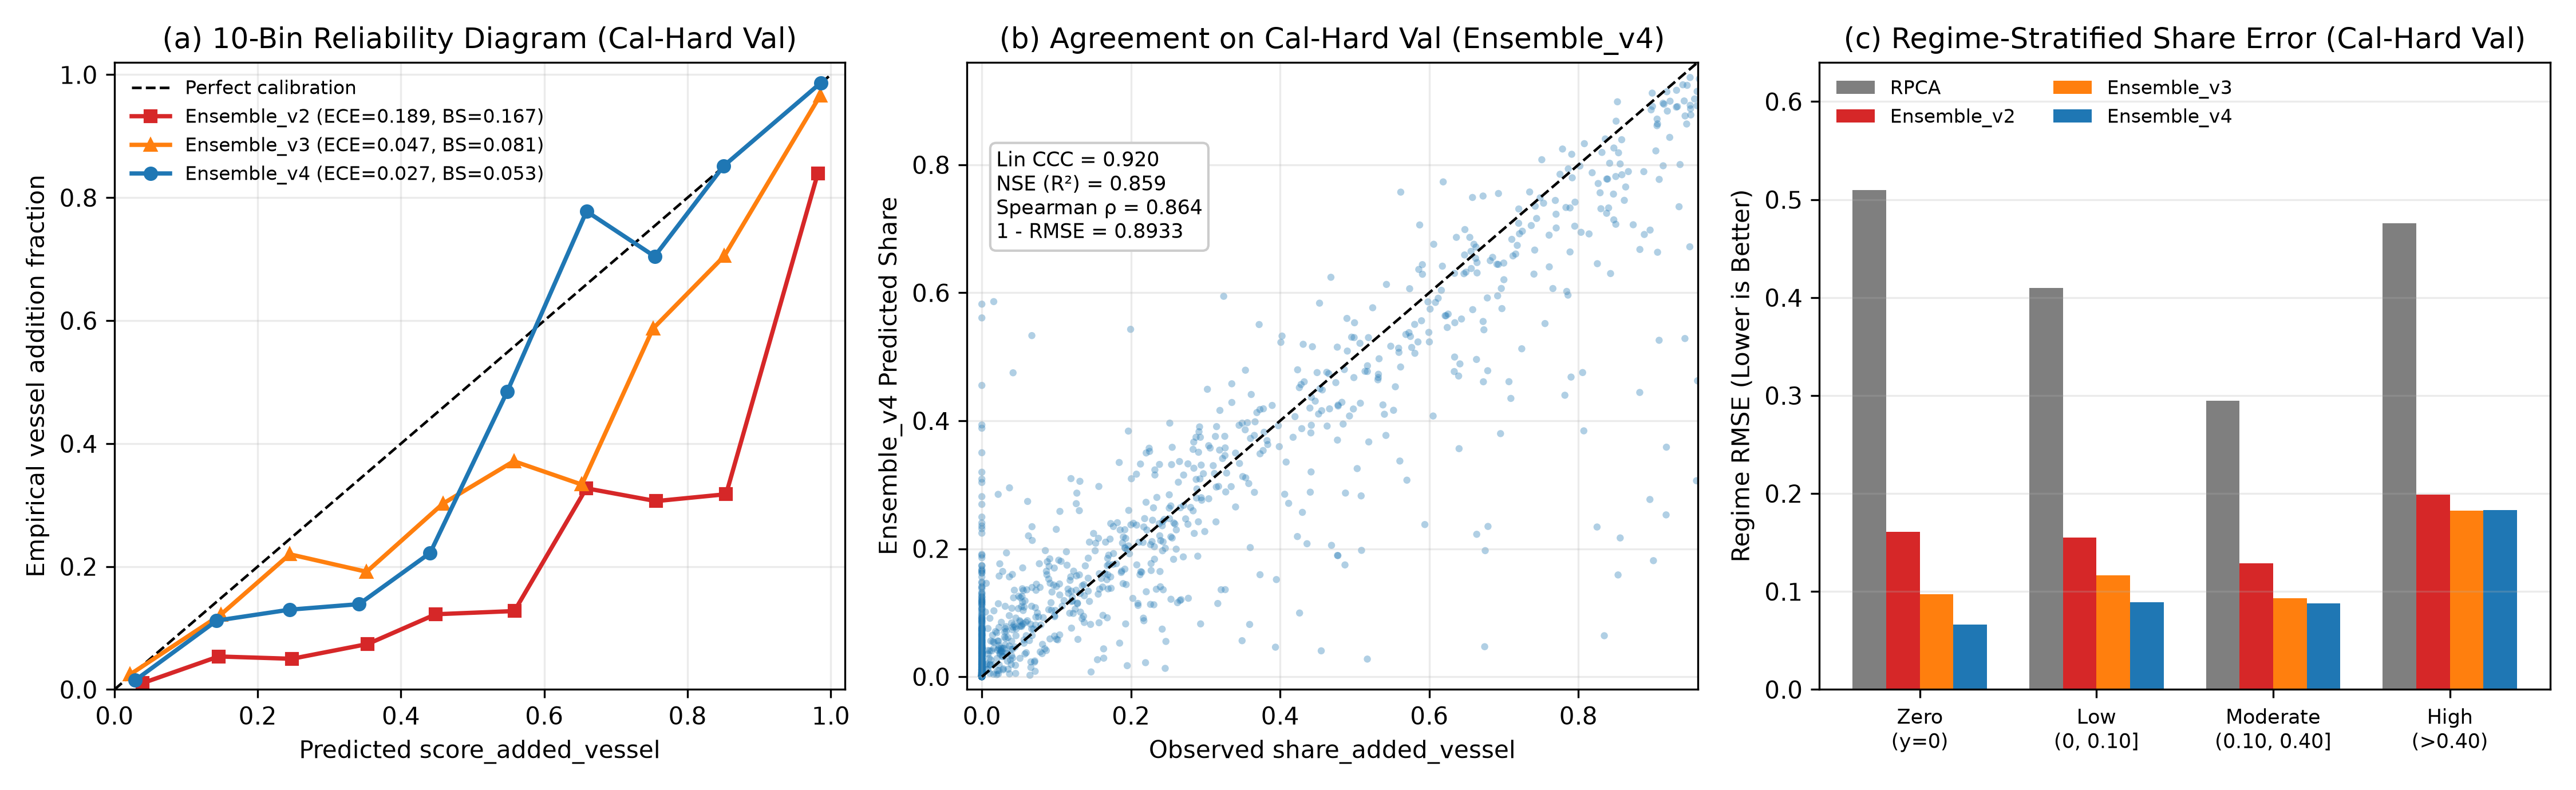
\includegraphics[width=0.84\textwidth]{figures/fig5_standards_calibration_and_agreement.png}
\caption{International standards evaluation: (a) 10-bin probability reliability curves and $\mathrm{ECE}_{10}$ on \texttt{val\_cal\_hard}; (b) predicted versus observed agreement with Lin's CCC, NSE, and Spearman $\rho$; and (c) regime-stratified share RMSE (\texttt{Zero}, \texttt{Low}, \texttt{Moderate}, \texttt{High}).}
\label{fig:standards_cal}
\end{figure}

\begin{table}[!htbp]
\centering
\caption{Unseen-station and five-stratum accuracy progression from \texttt{Ensemble\_v2} through \texttt{Ensemble\_v3} to \texttt{Ensemble\_v4}.}
\label{tab:strata}
\resizebox{\textwidth}{!}{%
\begin{tabular}{@{}llrrrrr@{}}
\toprule
Scope & Group / Stratum & $n$ & v2 ($1-\mathrm{RMSE}$ / AUC) & v3 ($1-\mathrm{RMSE}$ / AUC) & v4 ($1-\mathrm{RMSE}$ / AUC) & v4 Zero RMSE $\downarrow$ \\
\midrule
    Holdout Station & Fish Hoek (Unseen) & 297 & 0.8715 / 0.930 & 0.8739 / 0.947 & \textbf{0.9123} / \textbf{0.957} & \textbf{0.0395} \\
    Holdout Station & Sea Point (Unseen) & 244 & 0.9140 / 0.939 & 0.9358 / 0.992 & \textbf{0.9355} / \textbf{0.991} & \textbf{0.0231} \\
    Hard-Neg Stratum & Strict HF Ship & 899 & 0.8153 / 0.930 & 0.8815 / 0.956 & \textbf{0.8994} / \textbf{0.973} & \textbf{0.0803} \\
    Hard-Neg Stratum & VLF Surf Swell & 1141 & 0.8747 / 0.953 & 0.9006 / 0.973 & \textbf{0.9046} / \textbf{0.985} & \textbf{0.0339} \\
    Hard-Neg Stratum & Reef Biol. Chorus & 433 & 0.8967 / 0.966 & 0.9173 / 0.980 & \textbf{0.9177} / \textbf{0.987} & \textbf{0.0303} \\
    Hard-Neg Stratum & Telemetry Glitch & 280 & 0.8328 / 0.953 & 0.8941 / 0.991 & \textbf{0.9049} / \textbf{0.995} & \textbf{0.0496} \\
    Ambient Reference & Ambient Normal & 747 & 0.8527 / 0.924 & 0.8747 / 0.956 & \textbf{0.9029} / \textbf{0.971} & \textbf{0.0736} \\
\bottomrule
\end{tabular}%
}
\end{table}

\begin{figure}[!htbp]
\centering
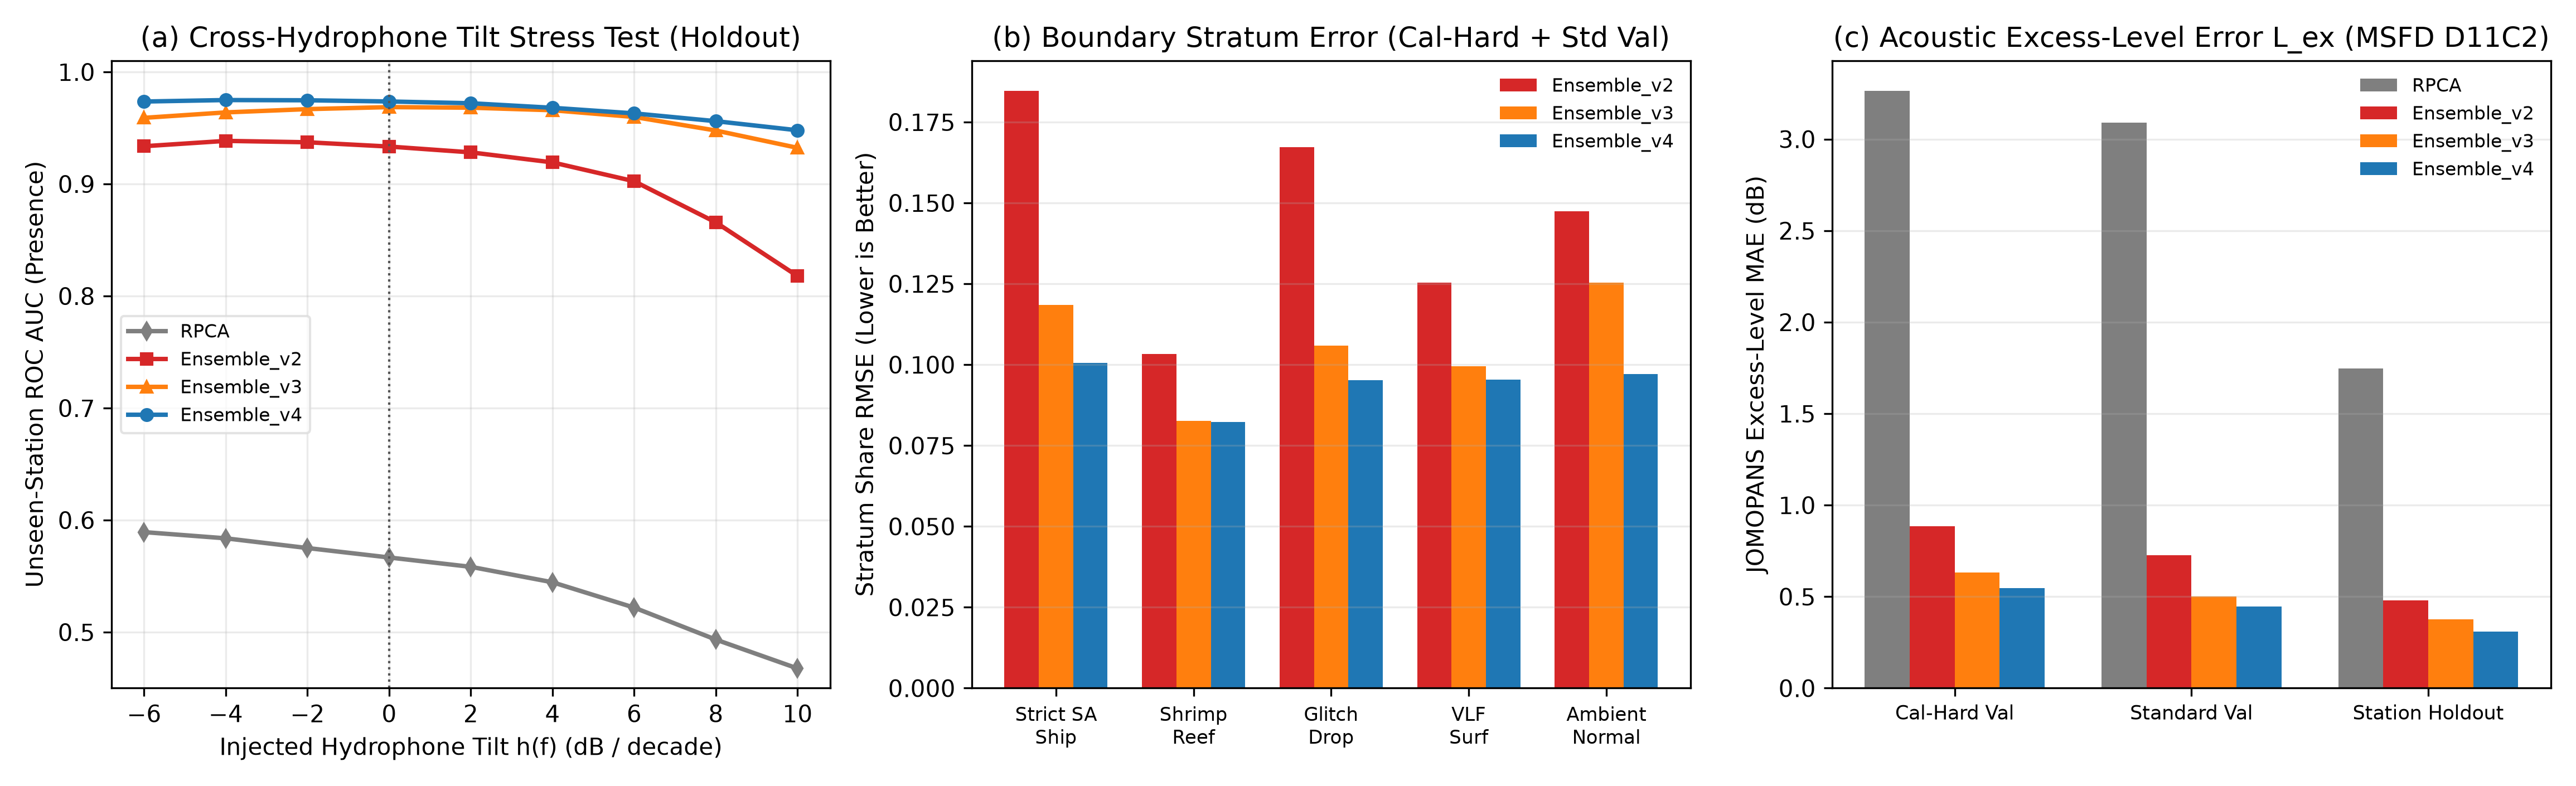
\includegraphics[width=0.84\textwidth]{figures/fig6_boundary_stress_and_calibration_shift.png}
\caption{Boundary stress tests: (a) unseen-holdout ROC AUC degradation under $-6$ to $+10$\,dB/dec hydrophone tilt; (b) error by South African hard-negative stratum; and (c) JOMOPANS/MSFD D11C2 excess-level MAE ($L_{\mathrm{ex}}$) across \texttt{val\_cal\_hard}, \texttt{val\_standard}, and \texttt{holdout}.}
\label{fig:boundary_stress}
\end{figure}

\begin{figure}[!htbp]
\centering
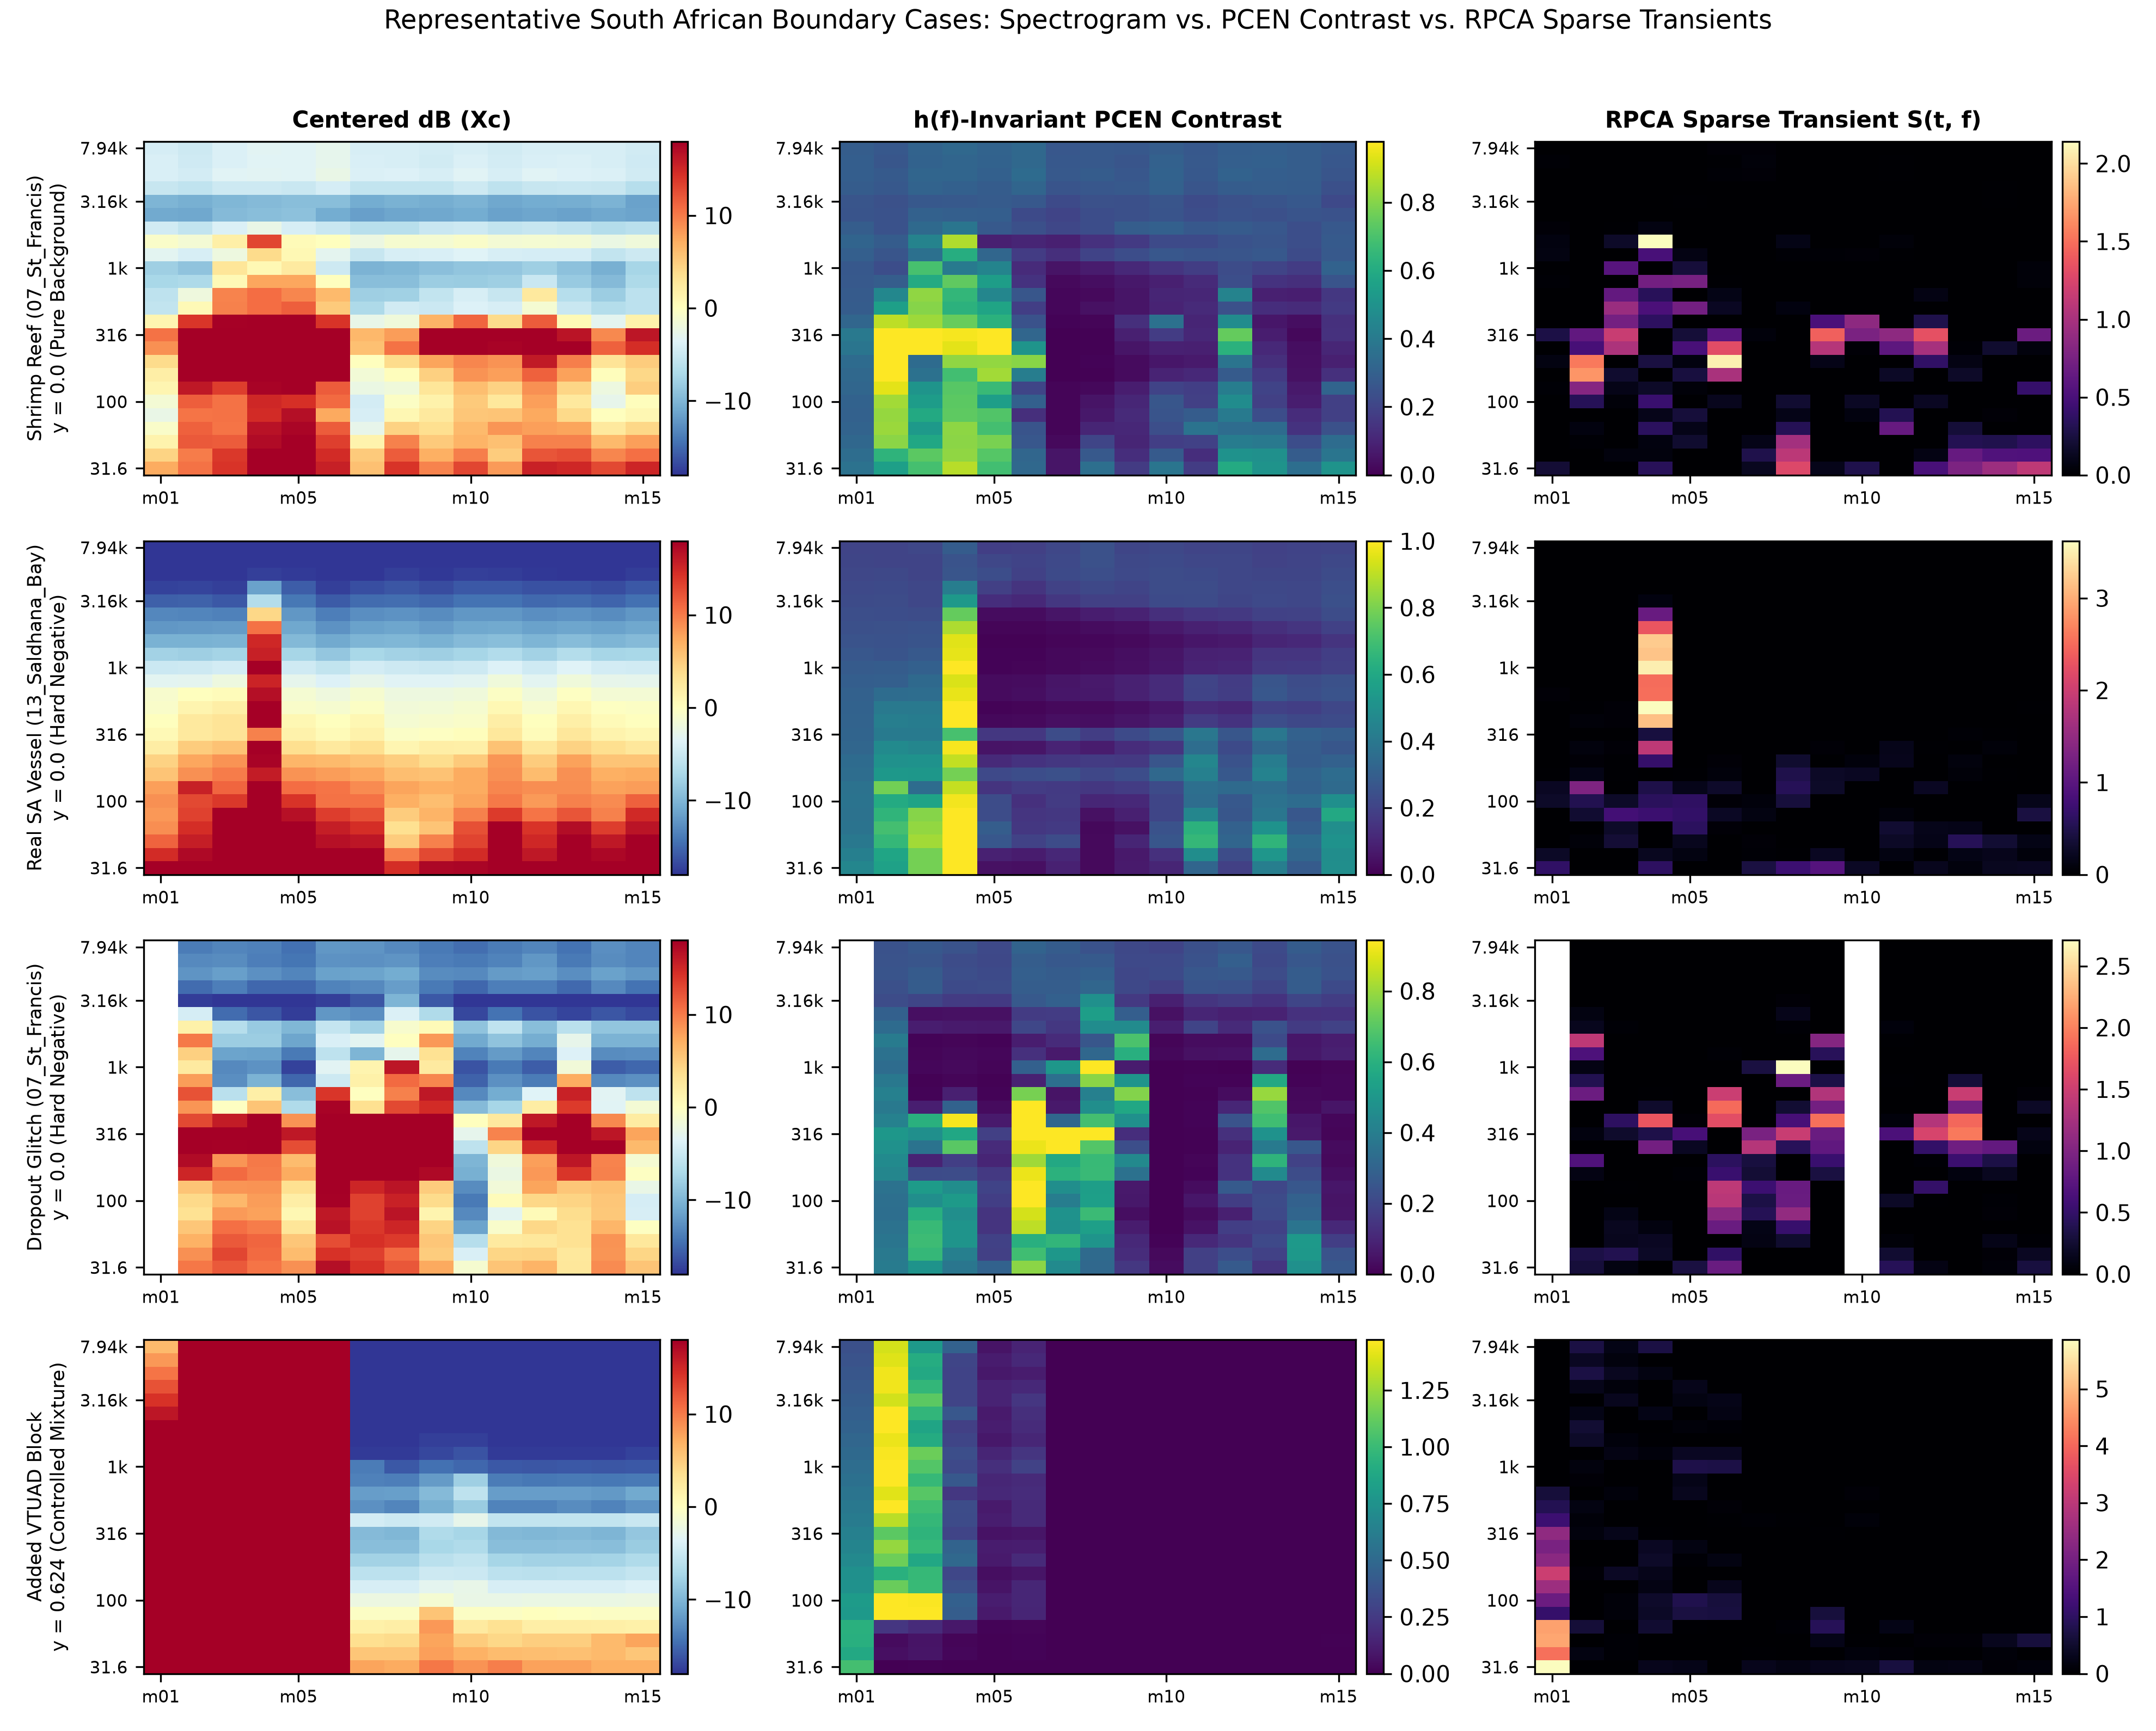
\includegraphics[width=0.77\textwidth]{figures/fig7_acoustic_signal_boundaries_decomposition.png}
\caption{Acoustic signal decomposition across three real South African hard negatives ($y=0$: shrimp reef, real SA vessel pass, dropout glitch) and a controlled VTUAD mixture ($y=0.624$), contrasting centered ISO~18405 spectra, PCEN contrast, and RPCA sparse transients.}
\label{fig:signal_decomp}
\end{figure}

\section{Evidentiary Boundaries, Domain-Generalization Contingency, and Reproducibility}

Three open measurement boundaries still constrain coastal inference across this dataset: (a) missing per-hydrophone sensitivity tables prevent converting uncalibrated exports to physical $\mathrm{dB\,re\,1\,\mu Pa}$ \parencite{iso2017underwater,robinson2014npl}; (b) candidate coordinates without verified deployment dates prohibit absolute shipping-density interpolation \parencite{ainslie2020adeon,farcas2020shipping}; and (c) zero synchronized field AIS logs exist in test windows. If Submission~\#3 (\texttt{submissions/candidate\_v4\_ensemble.csv}) still exhibits residual upward scoring bias on uncalibrated ports, my documented Modeling~v5 contingency isolates \texttt{score\_added\_vessel} strictly to exact $h(f)$-invariant \texttt{R\_*}, PCEN, and RPCA predictors combined with \texttt{ResNorm} \parencite{kim2021resnorm} and \texttt{Freq-MixStyle} \parencite{zhou2021mixstyle} normalization without spectral-tilt channel~4.

All results are bit-exact and auditable anytime across any clean Python~3.13 environment matching the 125 pinned non-AutoML packages in \path{requirements.txt} \parencite{breiman2001rf,ke2017lightgbm,chen2016xgboost,prokhorenkova2018catboost,he2016resnet}:
\begin{itemize}
    \item \textbf{Single-command verification and archives:} \path{scripts/reproduce_pipeline.py} (\texttt{-{}-mode verify-only}) validates environment pins, SHA-256 digests, and six independent deterministic self-tests (\texttt{v2}, \texttt{v3}, \texttt{v4\_simulator}, \texttt{v4\_features}, \texttt{v4\_train}, and \texttt{standardized\_evaluation\_suite}). Subprocess reloads of \path{models/v4/bundle_v4.joblib} (zero custom \texttt{\_\_main\_\_} classes) reproduce saved submissions within $\le 3.55 \times 10^{-9}$ share / $0.0$ score, while $+37.5$\,dB shifts yield $0.0$ holdout difference.
    \item \textbf{Reproducible notebooks and archives:} Three executed notebooks (\texttt{01} EDA/experiments, \texttt{02} V2 11-model benchmark, \texttt{03} \texttt{v2->v3->v4} generalization and standards) accompany the verified $<10$\,MB runnable code package \path{research_and_modeling_code_final.zip} (40 scripts, zero raw audio or competition test data) and preserved V6 science archive \path{research_code_v6.zip} (79620 bytes). External-data (\path{docs/EXTERNAL_DATA_DISCLOSURE.md}) and map disclosures remain archived, and \texttt{Test.csv} stayed strictly inference-only.
\end{itemize}

\section{Conclusion}

Tracing live leaderboard performance from Submission~\#1 (0.7615 / 0.5175 AUC) through \texttt{Ensemble\_v2} (0.7750 / 0.5484 AUC) exposed hydrophone frequency response $h(f)$ leakage and coastal ambient transients that clean multi-site synthetic splits initially concealed. By proving algebraic $h(f)$ cancellation in \texttt{Ensemble\_v4} via per-band temporal excess residuals $R(t,f)$, five-stratum South African hard negatives, and calibration-augmented 7-channel SE-ResNet blending, I lifted unseen-station accuracy to 0.9219 (0.9737 AUC, 0.0329 \texttt{zero\_rmse}), cut JOMOPANS excess error to 0.308\,dB, and maintained 0.9561 AUC under severe $+8$\,dB/decade hardware tilt while keeping measurement boundaries explicit.

\printbibliography[heading=bibintoc,title={References}]

\end{document}
